\chapter[Multimodaler Prototyp]{Umsetzung des multimodalen Prototyps}\label{cha:Prototyp}
Im nächsten Schritt sollen die Anwendungsbeispiele in geeigneter Weise umgesetzt werden, um in einer Studie Interaktionszeiten erheben zu können. 

Unser erster Ansatz war das Interface als Klickdummy zu erstellen und mit der "`Wizard of Oz"' Methode umzusetzen \citep{salber1993applying}. 
In der "`Wizard of Oz"' Methode simuliert der sogenannte "`Wizard"' die Funktionalität eines Systems, indem er Events durch seine Beobachtungen manuell auslöst. 
Das heißt die Funktionalität, bestimmte Gesten oder Sprachbefehle zu erkennen, muss in diesem Fall nicht implementiert werden und ist somit auch nicht anfällig für Fehler. 
Dies ist ein großer Vorteil für ein Modell, dass von Experten ausgeht, die mit dem System vertraut sind und keine Fehler machen. 
Auch Fehler des Systems können mit dieser Methode ausgeschlossen werden. 

Da in der "`Wizard of Oz"' Methode, Events nur durch den "`Wizard"' ausgelöst werden können, ist es schwieriger diese Events zu protokollieren. 
Studien dieser Art werden meist per Video aufgezeichnet und anschließend mit einer Videoanalyse ausgewertet. 
Natürlich gibt es einige Hilfen, um eine Videoanalysen zu optimieren, allerdings bleibt der Zeitaufwand hoch, weshalb wir uns dafür entschieden haben diese Methode nicht zu verwenden. 
Mit einem vollständig funktionsfähigem Prototypen können Events mit Zeitstempeln protokolliert werden, um später die Zeiten für unsere Aktionen und deren Wechselkosten berechnen zu können. 

Im folgenden werden die Anwendungsbeispiele und deren Implementation erläutert.

\section[Anwendungsbeispiele]{Beschreibung und Umsetzung der Anwendungsbeispiele}
Die im Workshop erarbeiteten Anwendungsbeispiele werden in vereinfachter und abstrakter Darstellung im Prototypen umgesetzt. 
Damit wollen wir vermeiden, dass ein auffälliges Design den Nutzer ablenkt. 
Es sollen lediglich die Interaktionszeiten untersucht werden und nicht eine bestimmte Umsetzung eines Interfacedesigns. 
In \fref{fig:UseCases} werden die Anwendungsbeispiele gezeigt welche im Folgenden beschrieben werden, ohne auf die Verwendung der Modalitäten einzugehen. 
Auf die Modalitäten gehen wir im Abschnitt Implementation unter der jeweiligen Modalität ein. 

Diese vier Anwendungsbeispiele sollen in der Studie sowohl unimodal, als auch mit allen multimodalen Kombinationen getestet werden. 
Jeder Proband kann sich in einem Probedurchgang mit der Aufgabe vertraut machen.
Anschließend folgen zwei Messdurchgänge, in denen die Interaktionszeiten erhoben werden. 

In \fref{fig:UseCases} werden die vier umgesetzten Anwendungsbeispiele in einer Übersicht horizontal dargestellt. 
Hier wird auch deutlich, ab welchen Screens ein Moduswechsel stattfinden soll. 
Der Moduswechsel wurde festgelegt und ist immer mit einem Screenwechsel verbunden. 
Durch diese Vorgabe ist unser Prototyp exklusiv redundant, da nur innerhalb eines Screens die Modalität gewechselt werden soll. 
\begin{figure}[ht]
  \centering
  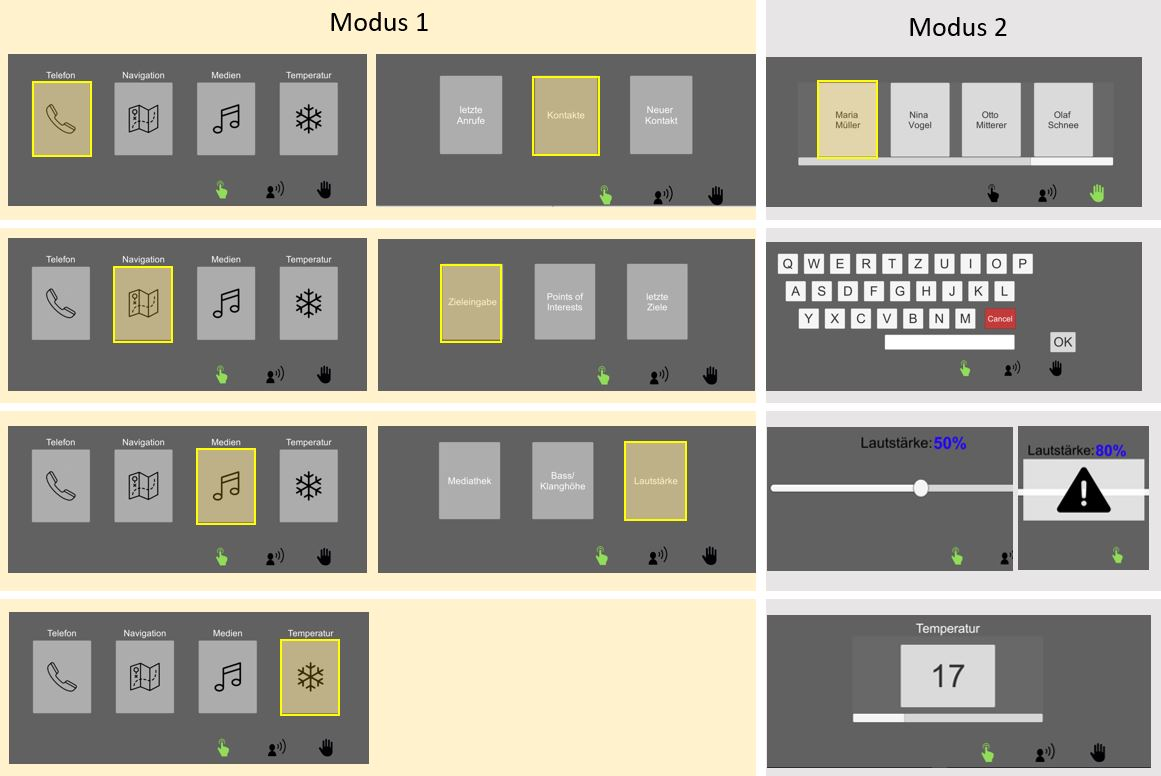
\includegraphics[width=1\textwidth]{img/UseCases2.jpg}
  \caption[Übersicht der Screenabfolge, der 4 Anwendungsbeispiele.]{Übersicht der Screenabfolge, der 4 Anwendungsbeispiele. Ein Anwendungsbeispiel besteht aus den horizontal abgebildeten Screens. Vertikal werden die Anwendungsbeispiele in ersten Modus und zweiten Modus geteilt. Dazwischen findet der Moduswechsel statt. Referenz zu den Icons siehe Kapitel \ref{cha:Danksagung}}
  \label{fig:UseCases}
\end{figure}

Im ersten Anwendungsbeispiel soll "`Maria Müller"' angerufen werden. Dafür muss im Hauptmenü die Kachel "`Telefon"' auf der linken Seite ausgewählt werden. 
Sobald diese Kachel mit einem Modus aktiviert wurde, wechselt der Screen in ein Untermenü mit drei Optionen, von denen die Kachel Kontakte auszuwählen ist. 
Jetzt muss durch eine horizontale Liste von Kontakten navigiert werden. 
Die Liste lässt sich seitenweise scrollen. 
Auf der dritten Seite befindet sich auf der linken Kachel der gewünschte Kontakt "`Maria Müller"', der auszuwählen ist. 
Dieses Anwendungsbeispiel besteht aus einer zweifachen Direktauswahl aus sichtbaren Elementen, einer Listennavigation bestehend aus drei Swipes gefolgt von einer Direktauswahl aus sichtbaren Elementen. 
Die Aktionen sind:
$$\textbf{2* \text{DA} + 3 * \text{L} + \text{DA}}$$

In der zweiten Anwendung soll zu einem von drei verschiedenen Zielen navigiert werden. 
Dazu wird im Hauptmenü die Navigationskachel ausgewählt und anschließend im nächsten Untermenü die Kachel Zieleingabe. 
Um das Ziel einzugeben ist eine vereinfachte Tastatur abgebildet, die im Touchmodus verwendet werden kann. 
Mit dem "`OK"' Button soll die Zieleingabe bestätigt werden. 
Hier bestehen die Aktionen aus zwei Direktauswahlen aus sichtbaren Elementen, einer Texteingabe und der Bestätigung. 
Die Aktionen sind:
$$\textbf{2 * \text{DA} + \text{Xmal Buchst.} + \text{B}}$$

In der dritten Anwendung soll die Lautstärke von 50\% auf 80\% erhöht werden. 
Dazu wird im Hauptmenü die Kachel "`Medien"' selektiert. 
Im darauf folgenden Untermenü ist die Kachel "`Lautstärke"' auszuwählen. 
Die Lautstärke muss mit einem horizontalen Slider auf einen Wert zwischen 75\% und 85\% gestellt werden. 
Dann erscheint eine Warnung als Popup, dass bestätigt werden muss. 
Auch hier setzt sich die Interaktion aus einer zweimaligen Direktauswahl aus sichtbaren Elementen, einer direkten Inkrementation des Sliders und einer Bestätigung zusammen.
Die Aktionen sind:
$$\textbf{2 * \text{DA} + \text{Inkr. (d)} + \text{B}}$$

Das letzte Anwendungsbeispiel hat zum Ziel die Temperatur von 17 auf 20 Grad zu erhöhen. 
Dazu muss im Hauptmenü die Kachel "`Temperatur"' selektiert werden. 
Die aktuelle Temperatur wird angezeigt und kann durch schrittweise Inkrementation einer horizontalen Liste erhöht werden.
Es ist jeweils nur ein Element der Liste, das heißt eine Temperatur, sichtbar.
Dieses Anwendungsbeispiel ergibt sich aus einer Direktauswahl aus sichtbaren Elementen und einer dreifachen Inkrementation des Wertes. 
Die Aktionen sind:
$$\textbf{\text{DA} + 3 * \text{Inkr. (s)}}$$

Das Anwendungsbeispiel "`Einen Song aus einer Liste auszuwählen"' wurde nicht umgesetzt, da ein weiteres  Anwendungsbeispiele die Studiendauer deutlich erhöht hätte. 
Außerdem ähnelt diese Interaktion sehr dem Anwendungsbeispiel einen Kontakt aus einem Liste zu wählen und hätte somit keinen wesentlichen Mehrwert. 
Wir werden dieses Anwendungsbeispiel für die Evaluation verwenden.

Die Direktauswahl aus sichtbaren Elementen wurde immer im ersten Modus ausgeführt.
Anschließend folgt ein Moduswechsel. 
Die drei möglichen Modalitäten wurden mit kleinen schwarzen Symbolen für Touch, Sprache und Geste in jedem Screen angezeigt. 
Der Modus, den der Proband verwenden soll wurde grün hervorgehoben. 
In \fref{fig:ModusAktiv} soll beispielsweise mit dem Modus Touch interagiert werden. 
\begin{figure}[ht]
  \centering
  
\includegraphics[width=0.5\textwidth]{img/ModusAktiv.jpg}
  \caption[Symbolische Anzeige des aktiven Modus]{Symbolische Anzeige des aktiven Modus, der von den Probanden ausgeführt werden soll. Referenz zu den Icons siehe Kapitel \ref{cha:Danksagung}}
  \label{fig:ModusAktiv}
\end{figure}

Ist die Modalität Geste aktiv, haben wir eine zusätzliche Information in die Gestensymbolik eingebaut. 
In der aktiven grünen Hand ist ein Punkt zu sehen, der wie bei einer Ampel entweder rot, gelb oder grün ist. 
Dieser Punkt dient dazu besser erkennen zu können, ob und wo die rechte Hand vom Leap Motion Controller erkannt wird. 
Wie in \fref{fig:Ampeldarstellung} zu sehen ist, ist der Punkt rot, wenn die Hand von dem Controller nicht erkannt wird. 
Wird die Hand vom Controller erkannt, befindet sich aber nicht im Interaktionsbereich, indem Gesten ausgeführt werden können, ist der Punkt gelb.
Grün wird der Punkt, sobald die Hand erkannt wurde und sich im Interaktionsbereich befindet.
\begin{figure}[ht]
  \centering
  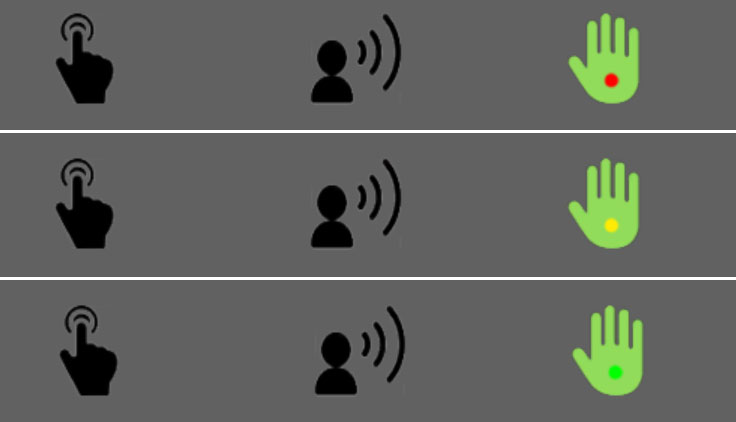
\includegraphics[width=0.5\textwidth]{img/Gestenerkennung.jpg}
  \caption[Ampeldarstellung zur Gestenerkennung]{Ampeldarstellung zur Gestenerkennung. Der rote Punkt bedeutet, das die rechte Hand vom Leap Motion Controller nicht erkannt wurde. 
	Gelb wird der Punkt, wenn die Hand erkannt wurde, sich aber nicht im Interaktionsbereich befindet. 
	Grün ist der Punkt wenn sich die Hand im Interaktionsbereich befindet. Referenz zu den Icons siehe Kapitel \ref{cha:Danksagung}}
  \label{fig:Ampeldarstellung}
\end{figure} 
Mit dieser Visualisierung soll für den Beobachter veranschaulicht werden, falls Gesten nicht erkannt wurden. 

Wird ein Button angewählt bekommt dieser eine gelbe Markierungsfarbe. 
Bei einer Selektion bekommt der Nutzer ein zusätzliches Audio Feedback eines Klickgeräuschs.

\section[Implementation]{Implementation des multimodalen Prototypen}
Der multimodale Prototyp wurde in Unity (Version 5.4 \citep{Unity}) auf einem Surface umgesetzt, was die Touch Interaktion ermöglicht. 
Für die Gestenerkennung wird ein Leap Motionen Controller \citep{Leap} verwendet. 
In Unity wurde ein Software Developer Kit namens Orion \citep{OrionBeta} verwendet, welches in die Unity Szene eingebunden wird. 
Um die Spracherkennung zu gewährleisten wurde in Unity ein Skript eingebunden, dass auf die Windows integrierte Spracherkennung zugreift. 
Die Skripte wurden mit Visual Studio in C\# geschrieben.

Jeder Screen wurde in Unity in eine eigene Szene eingebaut.
Die Selektion eines Buttons durch ein Touch-Event, eine Selektionsgeste oder durch einen Sprachbefehl, lädt die nächste Szene. 
Im ersten Screen wird vom Versuchsleiter die Proband ID eingetragen und die passende Permutation geladen (mehr zur Permutation siehe Kapitel \ref{cha:Studie}). 
In der Permutation steckt das aktuelle Anwendungsbeispiel, sowie die zu verwendenden Modalitäten. 
Die permutierte Reihenfolge der Kombinationen verhindert das eventuell enstandene Lerneffekte unsere Messungen beeinflussen. 

Der Versuchsleiter kann mit den Pfeiltasten einer externen Tastatur das nächste Anwendungsbeispiel laden, einen Messdurchgang aktiviert und den Durchgang gestartet.  
Zur Vorbereitung wird als erstes ein schwarzer Screen für drei Sekunden gezeigt.
Anschließend wird der Hauptscreen geladen, mit dem die Interaktion beginnt.

Um Fehler zu reduzieren ist es mit den Modalitäten Geste und Sprache nicht möglich eine falsche Auswahl zu tätigen. 
Wir haben uns entschieden für die Sprache keinen Push To Talk Button zu verwenden, da wir Aktionszeiten messen wollen und wir uns auf die Modalitäten Touch, Geste und Sprache fokussieren. 
Sollter dieser haptische Knopfdruck verwendet werden, müsste die Zeit für diese Aktion hinzugefügt werden.  

\subsection[Touch]{Realisierung der Toucheingabe} 
\citet{Wobbrock:2009} untersucht von Nutzern definierte Touchgesten auf einem Surface. 
Sie fanden heraus, dass die Anzahl der Finger für eine Touchgeste für die meisten Nutzer irrelevant ist und das einhändige Touchgesten bevorzugt werden. 
Bei unseren Touchgesten entschieden wir uns für drei verschiedene Touchgesten (siehe \fref{fig:TouchGestures}):
\begin{itemize}
\item Einen direkten Touch (Tap), um einen Button auszuwählen. 
Die Selektion geschieht erst wenn der Finger den Touchscreen verlässt. 
\item Eine Swipegeste, um eine Liste seitenweise zu scrollen oder einen Wert zu inkrementieren.
\item Eine direkte Inkrementation des Slides, um den Wert des Sliders zu verstellen (Slidegeste).
Hierbei wird der Regler des Slider ähnlich wie bei Drag and Drop direkt verschoben, allerdings nur entlang des Achse des Sliders.
Der Finger bleibt während der Verschiebung auf der Touchfläche.
\end{itemize}
In der \ref{fig:TouchGestures} sind die 3 Varianten veranschaulicht.
\begin{figure}
	\centering
		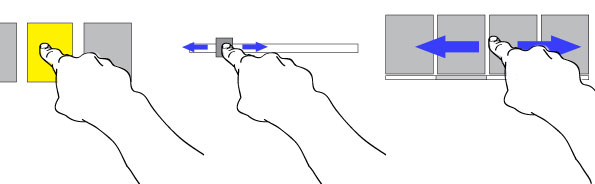
\includegraphics[width=1\textwidth]{img/TouchGestures.jpg}
	\caption{Touchgesten: Tap, Slidegeste und Swipegeste für die Toucheingabe}
	\label{fig:TouchGestures}
\end{figure}

\subsection[Geste]{Realisierung der Gesteneingabe}
Auch bei der Erkennung der Gesten wurden drei verschiedene Arten implementiert. 
Um einen Button zu selektieren wird zuerst geprüft, ob sich eine rechte Hand im festgelegten Interaktionsbereich befindet. 
Dieser Interaktionsbereich ist je nach Anzahl der Buttons in drei oder vier Bereiche entlang der x-Achse unterteilt. 
Je nachdem in welchem Bereich sich die Hand befindet ändert der passende Button dieses Bereichs die Farbe zu gelb.
Dies entspricht der Markierungsfarbe. 
Somit erkennt der Nutzer welcher Button gerade angewählt ist. 
Um einen Button nun zu selektieren, muss der Zeigefinger schnell nach unten bewegt werden, ohne dabei die Hand zu bewegen. 
Nur wenn ein entsprechender Button gelb markiert ist und die Selektionsgeste mit dem Zeigefinger ausgelöst wurde, wird dieser Button selektiert und somit die nächste Szene geladen. 

Die nächste Geste ist eine Wischgeste, um in einer Liste seitenweise zu scrollen oder einen Wert zu inkrementieren.
Das entspricht unseren Aktionen (L) und (Inkr. (s)). 
Diese Geste wurde in den Anwendungsbeispielen verwendet, um die Temperatur zu verändern und um die Liste der Kontakte zu durchsuchen. 
Wie zuvor muss die rechte Hand erkannt werden und sich im Interaktionsbereich befinden. 
Wenn sich die Hand entlang der x-Achse mit mindestens 80 Millimeter pro Sekunde von rechts nach links bewegen, löst dies eine Animation aus, die zur nächsten Seite navigiert. 
Damit die Hand nicht unbeabsichtigt zwei Seiten auf einmal oder direkt hintereinander scrollen lässt, wird die Erkennung der Wischgeste nach jeder Erkennung für eine Sekunde deaktiviert. 

Die dritte und letzte Geste ist eine Geste, um einen Slider zu verstellt. 
Hierfür müssen sich Daumen und Zeigefinger berühren und somit einen geschlossenen Kreis über dem Leap Motion Controller bilden.
Damit dieser Kreis von der Leap erkannt wird, ist es wichtig die anderen Finger abzuspreizen, siehe \ref{fig:Gestures}. 
Ist dieser Kreis geschlossen wird der Slider aufgenommen und kann verschoben werden. 
Um den Slider nach rechts oder links zu verstellen muss die Geste entlang der x-Achse durch Bewegung der Hand in eben diese Richtung verändert werden. 
Ist der gewünschte Wert erreicht, muss der Kreis geöffnet werden, indem sich Zeigefinger und Daumen wieder lösen. 
\begin{figure}
	\centering
		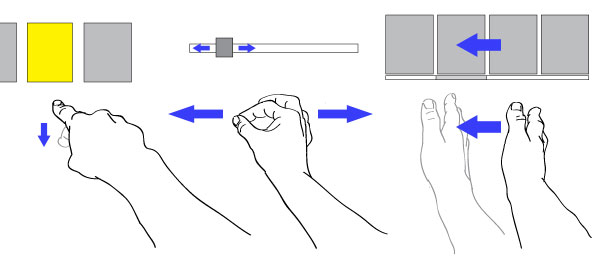
\includegraphics[width=1\textwidth]{img/Gestures-mit_Pfeile.jpg}
	\caption{Selektionsgeste, Slidegeste und Swipegeste}
	\label{fig:Gestures}
\end{figure}

\subsection[Sprache]{Realisierung der Spracheingabe}
Um die Spracherkennung zu ermöglichen wurden in Unity in jeder Szene die dementsprechenden Sprachbefehle als String definiert. 
Im Beispiel des Hauptscreens waren dies die Sprachbefehle: "`Telefon"', "`Navigation"', "`Medien"' und "`Temperatur"'. 
Die in Windows integgriert Spracherkennung verarbeitet gesprochene Befehle zu Strings.
Stimmt Strings mit einem der vordefiniertem String überein wird der passende Button selektiert. 

Damit der Nutzer bei der Direktauswahl aus sichtbaren Elementen zusätzlich zum Soundgeräusch Feedback bekommt wird der selektierte Button vor dem tatsächlichen Klick farblich gelb hervorgehoben. 
Um diesen Effekt erzielen zu können musste eine Verzögerung von einer halben Sekunden eingebaut werden.

Im Beispiel der Listen wird zur Veranschaulichung erst zum entsprechenden Wert geswiped, das heißt eine Animation ist sichtbar und anschließend wird die Kachel selektiert. 
Im Beispiel der Texteingabe wird das Inputfeld mit dem gesprochenen Ziel aktualisiert.

\subsection[Protokollierung]{Protokollierung der relevanten Events}
Um die Interaktionszeiten messen zu können werden die relevanten Aktionen mit Zeitstempeln in einer Textdatei protokolliert (Logdatei). 
Diese Logdatei ist so strukturiert, dass Werte durch Tabs separiert sind, um später in Excel leichter bearbeitet werden zu können.
An relevanten Stellen im Code wird die Logdatei geöffnet und der Zeitstempel zusammen mit dem Event in die Datei geschrieben und wieder geschlossen. 
Zur Veranschaulichung ist in \fref{fig:Auszug_Logging_Sound_TT} ein Auszug des Protokolls zusehen. 
Die Logdatei wurde hier bereits angepasst und in Excel als Tabelle formatiert (mehr dazu in Kapitel \ref{cha:Studie}). 
\begin{figure}
	\centering
		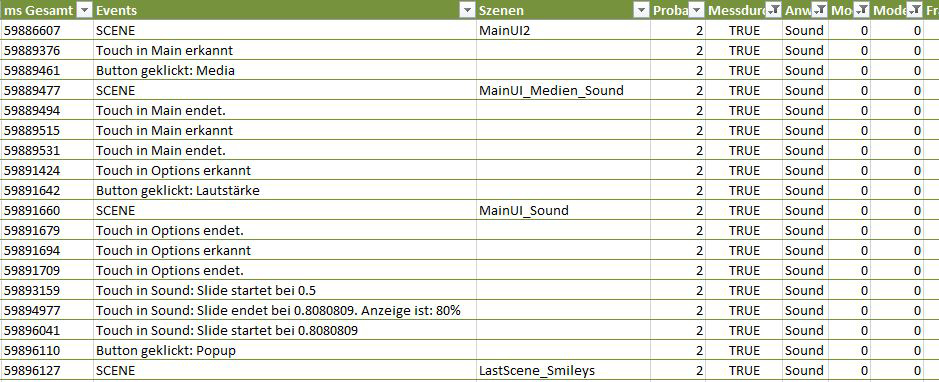
\includegraphics[width=1\textwidth]{img/Auszug_Logging_Sound_TT.JPG}
	\caption[Ausschnitt aus der Logdatei vom Anwendungsbeipiel Lautstärke]{Ausschnitt aus der Logdatei vom Anwendungsbeipiel Lautstärke, das mit den Modalität Touch und Touch, also unimodal ausgeführt wurde}
	\label{fig:Auszug_Logging_Sound_TT}
\end{figure}

Sobald ein Anwendungsbeispiel startet werden die Einstellungsinformationen siehe \fref{fig:ProbandenSettings} protokolliert. 
Diese enthalten die ID des Probanden, das aktuelle Anwendungsbeispiel, die zu verwendenden Modalitäten und ob es sich um einen Probe- oder um einen Messdurchgang handelt. 
Nach jedem Messdurchgang werden die Antworten protokolliert, die die Probanden über Eignung und Gefallen der gerade ausgeführten Moduskombination eingaben. TODO(smileys erwähnen bzw. Erläuterung hier einbauen)
Nach jedem Durchgang erscheint wieder der Einstellungsscreen, indem der Versuchsleiter das nächste Anwendungsbeispiel laden oder den Messdurchgang aktiviert kann. 
Für jede Runde werden die entsprechenden Infos vom Setting protokolliert.
\begin{figure}[ht]
  \centering
  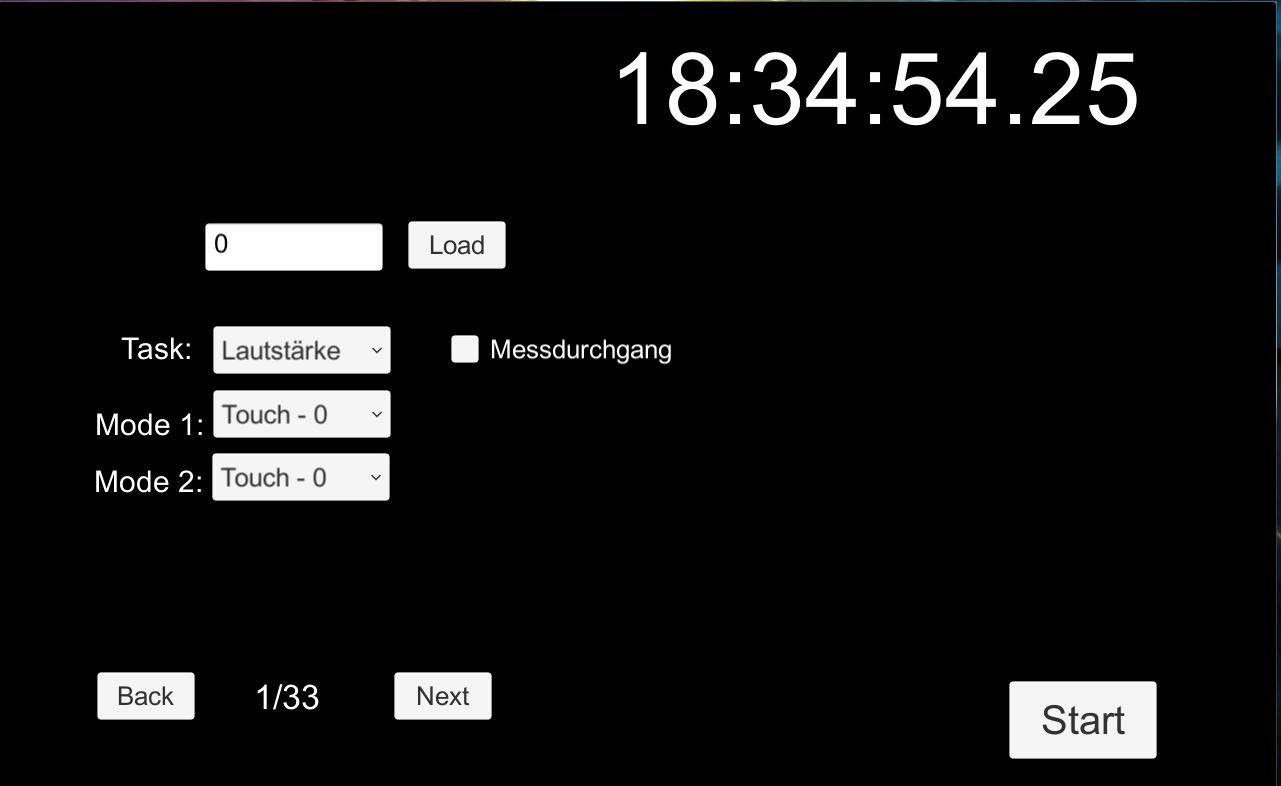
\includegraphics[width=1\textwidth]{img/SettingsPrototyp.jpg}
  \caption{Einstellungen vor jedem Durchlauf}
  \label{fig:ProbandenSettings}
\end{figure} 

Während des Anwendungsbeispiels wird der aktuelle Screen protokolliert, sobald er sichtbar geladen wurde. 
Jeder Touch, jede erkannte Geste und jeder erkannte Sprachbefehl wird ebenfalls protokolliert. 
Außerdem wird bei Listen die aktuelle Seite und beim Slider die Start- und Endwerte während einer Bewegung durch Touch oder Geste protokolliert. 
Bei jedem Button wird der Name des Buttons protokolliert, sobald der Button ausgelöst wurde. 
Mit diesen Logzeiten sollen nach der Studie die Zeiten der Operatoren berechnet werden. 
Dazu mehr in Kapitel \ref{cha:Studie}.  
